\section{Model and numerical methods}
\label{sec:methods}

\subsection{Hamiltonian and isolated-cell projection}

The Hamiltonian is
\begin{align}
H={}&J_1\sum_n\left(\bm S_{n,2}\!\cdot\!\bm S_{n,3}
 +\bm S_{n,3}\!\cdot\!\bm S_{n,4}\right) \notag\\
&+J_2\sum_n\left(\bm S_{n,1}\!\cdot\!\bm S_{n,2}
 +\bm S_{n,4}\!\cdot\!\bm S_{n,5}\right) \notag\\
&+J_3\sum_n\bm S_{n,5}\!\cdot\!\bm S_{n+1,1}.
\label{eq:hamiltonian}
\end{align}
The isolated pentamer has a 32-dimensional Hilbert space.
We diagonalize it completely and resolve each degenerate energy subspace by total spin and reflection parity.
Spectral weights are evaluated with projectors onto complete multiplets, avoiding the arbitrary orientation of individual eigenvectors within a degenerate subspace.

If $P$ projects onto the ground-state doublet, the local spins satisfy
\begin{equation}
P\bm S_{n,a}P=c_a\bm T_n,
\label{eq:projection}
\end{equation}
where $\bm T_n$ is an effective spin-$1/2$ operator.
To leading order in the inter-cell coupling,
\begin{equation}
\Heff=NE_5+\Jeff\sum_n\bm T_n\cdot\bm T_{n+1}+O(\beta^2),
\qquad \Jeff=\beta c_1c_5.
\label{eq:effective}
\end{equation}
We test the projection using exact diagonalization of two coupled pentamers and finite-chain calculations with $N=8,12,16$ pentamers.

\begin{figure*}[t]
  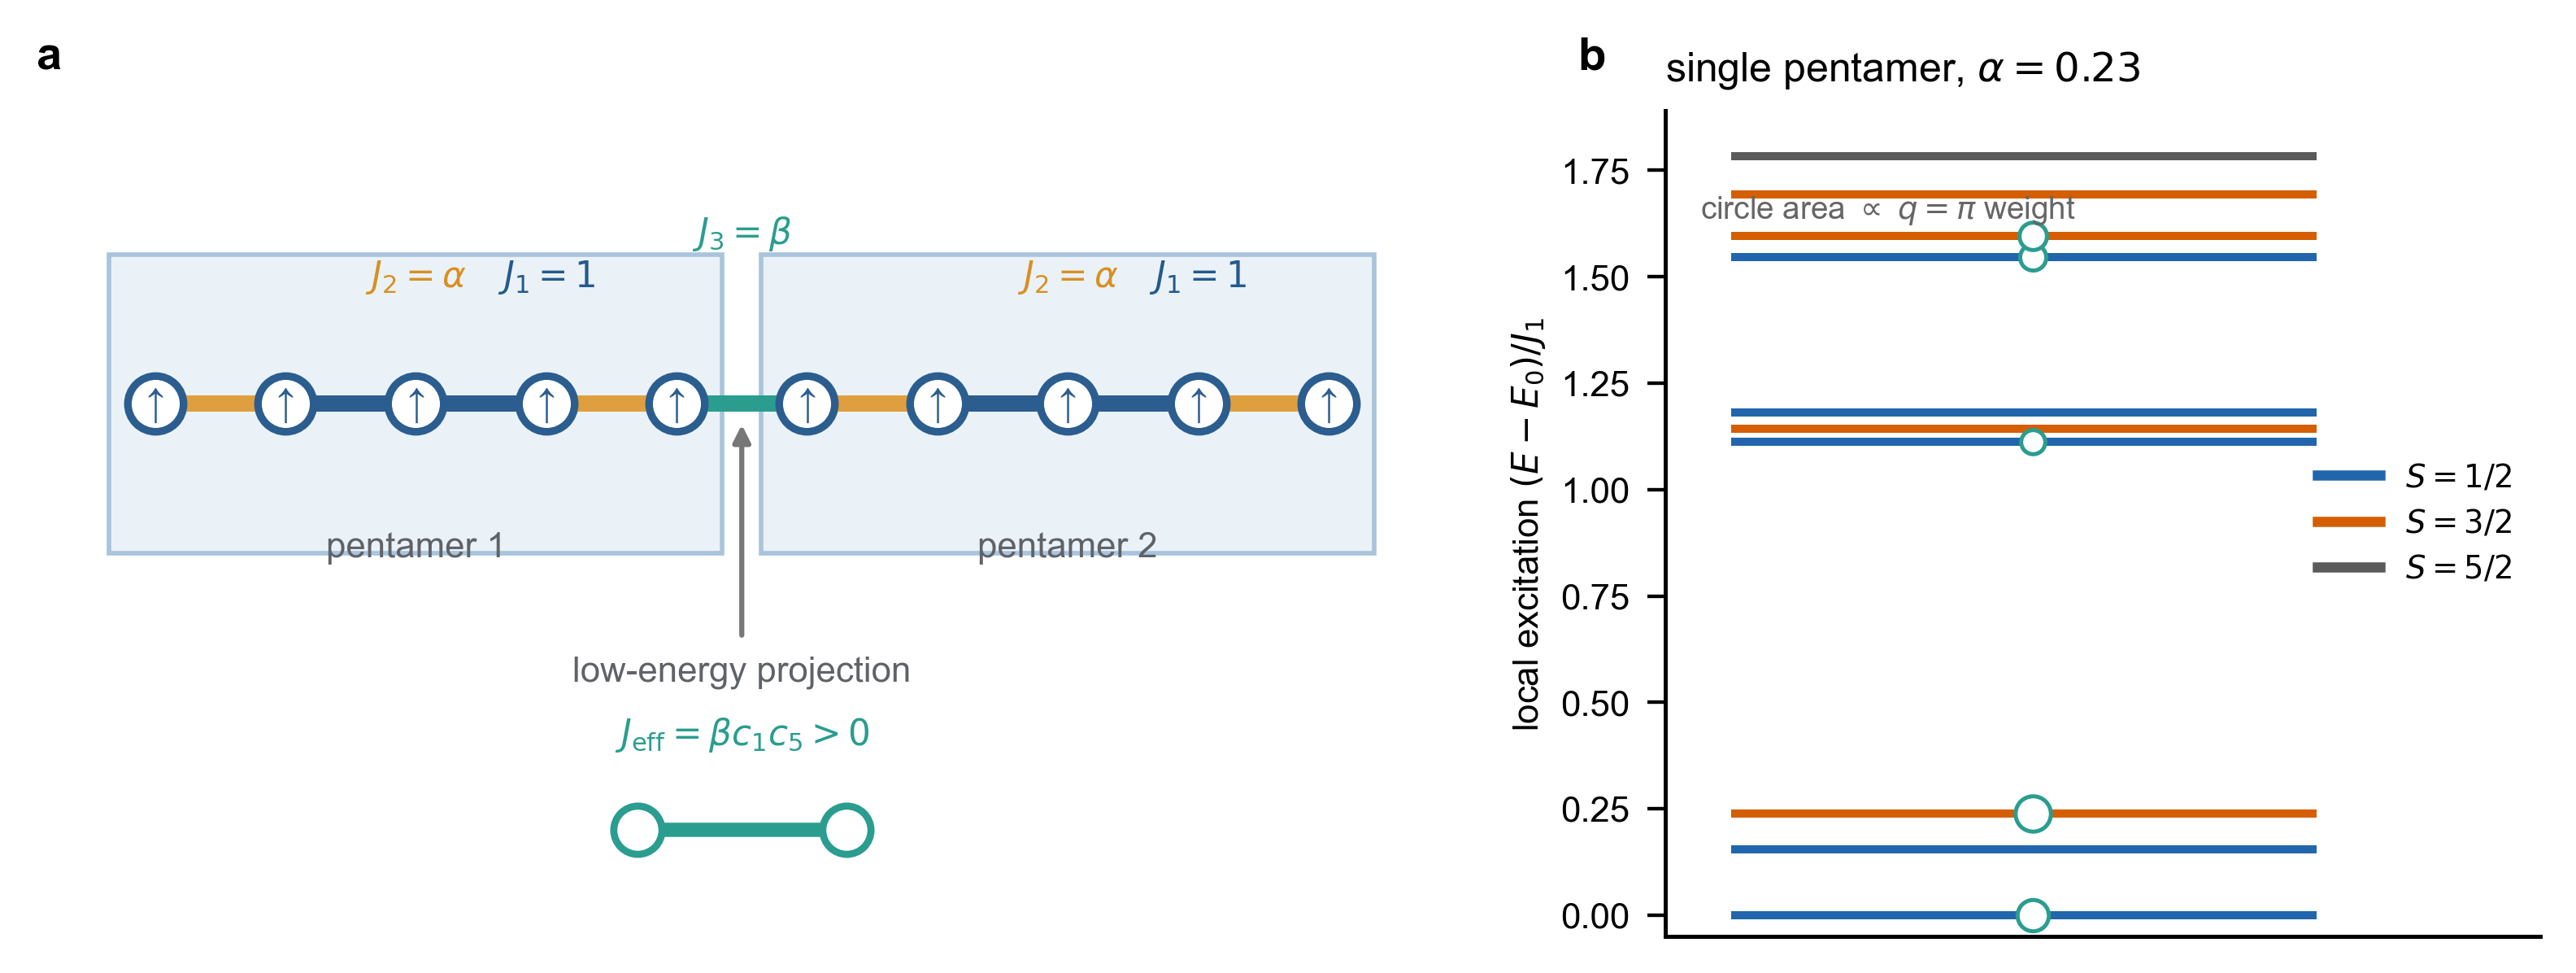
\includegraphics[width=\textwidth]{fig1_model_projection.png}
  \caption{Model and low-energy projection.
  The five-site unit cell defines the couplings $J_1$, $J_2$, and $J_3$.
  Isolated-pentamer multiplets are resolved by total spin and reflection parity, and the ground-state doublet is projected onto an effective spin-$1/2$ degree of freedom.}
  \label{fig:model}
\end{figure*}

\subsection{Static finite-chain calculations and acceptance gates}

Finite chains use open boundaries and $L=5N$ physical spins.
Ground states are obtained in fixed total-$S^z$ sectors with density-matrix renormalization group calculations in a matrix-product-state representation~\cite{white1992,schollwoeck2011}.
Sector-specific initial states are used rather than assuming that one initialization samples every low-energy solution.

The positive-region data set contains 105 accepted records at $L=40,60,80$.
For negative $\alpha$, the Practical V2 protocol uses the \texttt{center} and \texttt{ferro\_j2} product-state initializations in the $S^z=0$ sector and a fixed \texttt{center} initialization in the $S^z=1$ sector.
A new record is accepted only if
\begin{align}
\frac{\mathrm{Var}(H)}{L}&\leq5\times10^{-8}, \notag\\
\epsilon_{\mathrm{trunc}}&\leq10^{-9}, \notag\\
|S^z-S^z_{\mathrm{target}}|&\leq10^{-8},
\label{eq:gates}
\end{align}
and the sector gap is no smaller than $-10^{-8}$.
New Practical V2 calculations use at most 64 sweeps.
The two $S^z=0$ initial states test initialization sensitivity and are not independent statistical replicates.

Every accepted remote result is checked by parent and child manifests, transferred without overwriting earlier runs, checked again locally, and passed through an independent validator.
Records that fail a gate are retained as bounded or not evaluable and are excluded from accepted-only boundary inference.

\subsection{Entanglement, correlation, and momentum diagnostics}

For an open critical chain, the bond entropy is compared with
\begin{equation}
S(b)=a_g+\frac{\ceff}{6}
\ln\left[\frac{2L}{\pi}\sin\left(\frac{\pi b}{L}\right)\right].
\label{eq:entropy}
\end{equation}
The intercept $a_g$ depends on the bond class $g=b\bmod 5$ or $b\bmod 10$, while a common slope defines the descriptive coefficient $\ceff$.
Fits use central windows $fL\leq b\leq(1-f)L$ with $f=0.10$, 0.15, 0.20, and 0.25.
We call this quantity an effective entropy coefficient rather than a central charge unless size and solver controls justify the stronger interpretation~\cite{calabrese2004}.

The negative-$\alpha$ scan tracks the dominant structure-factor momentum $\qpeak$ and a dominant-ratio observable $R_L$.
A candidate boundary is retained only when an adjacent coupling interval shows both a momentum reconstruction and a consistent finite-size signature in $\Delta R=R_{80}-R_{60}$.

\subsection{Dynamical structure factor}

We compute the dynamical structure factor by two independent matrix-product-state routes.
Correction-vector DMRG gives a fixed-frequency spectrum at $q=\pi$~\cite{kuehner1999}.
Real-time evolution followed by Fourier transformation provides the full momentum dependence and an independent line-shape check~\cite{vidal2004,fishman2022}.
The correction-vector implementation reproduces the complete $L=10$ spectrum with relative $L_2$ error $8.52\times10^{-12}$.

The production full-momentum calculations use $L=40$, $t_{\max}=30$, 121 momentum points, 301 frequency points, and paired time steps $\Delta t=0.025$ and 0.0125.
The raw Fourier matrices, including negative ringing from the finite time window, are retained and tested rather than clipped.

\subsection{Krylov-subspace stability control}

The saved-state anomaly at $(\alpha,\beta)=(-0.10,0.25)$ was the point most sensitive to the local eigensolver configuration.
We therefore performed an $L=80$ control in which all physical and DMRG settings were fixed while the Krylov dimension increased from $k=8$ to 12.
Both $S^z=0$ initial states used 64 sweeps, configured maximum bond dimension 1200, cutoff $10^{-11}$, and the same 401-point momentum grid.
The symbol $k$ denotes the Krylov-subspace dimension and is distinct from the MPS bond dimension $\chi$.

The $k=12$ run passed the remote and local checksum chain and the Practical V2 validator.
Its variance per site was $1.86$--$1.87\times10^{-11}$, and the two sector gaps were $7.2772047002\times10^{-5}$ and $7.2772051798\times10^{-5}$.
Across 172 matched records, the $k=8\rightarrow12$ differences were bounded by $7.5211\times10^{-12}$ for the spin gap, $8.3994\times10^{-8}$ for the dominant ratio, and $5.7413\times10^{-8}$ for the entropy.
The value $\qpeak/\pi=1$ was unchanged.
The bond dimensions actually retained at this size were well below the configured cap and nearly insensitive to the solver change: the largest link dimension was 264--265 in the $S^z=0$ sector and 186--190 in $S^z=1$, against a configured maximum of 1200.

Two disclosures bound how these controls may be combined.
First, the $k=3\rightarrow8$ comparison is a solver-control audit, not a convergence proof, and the observed link dimensions are not a convergence statement: $k$ is the Krylov dimension, the retained bond dimension is $\chi$, and no $\chi$ series was performed.
Second, the historical negative-$\alpha$ records, including the $L=40$ and $L=60$ entries of the size comparison in Sec.~\ref{sec:results}, were produced with the earlier Krylov configuration; only the $L=80$ endpoint carries a $k=8$ control.
Records with different solver settings are therefore not combined into a finite-size scaling series, and no thermodynamic extrapolation is drawn from them.
